\documentclass[journal,12pt,twocolumn]{IEEEtran}
\usepackage[utf8]{inputenc}
\usepackage{amsmath}
\usepackage{amssymb}
\usepackage{graphicx}
\providecommand{\brak}[1]{\ensuremath{\left(#1\right)}}

\title{Assignment 3}
\author{ADEPU VASISHT}
\date{March 2021}


\begin{document}

\maketitle

\section*{GATE 2019(IN) Q.No 27(Eng section)}
The function $p\brak{x}$ is given by $p\brak{x} = \frac{A}{x^\mu}$ where $A$ and $\mu$ are constants with $\mu>1$ and $1\leq x<\infty$ and $p\brak{x}= 0$ for $-\infty<x<1$. For $p\brak{x}$ to be a probability distribution function, the value of A should be equal to?

\begin{description}
\item[$\brak{A}$]$\mu -1$\\
\item[$\brak{B}$]$\mu+1$\\
\item[$\brak{C}$]$\dfrac{1}{\mu-1}$\\
\item[$\brak{D}$]$\dfrac{1}{\mu+1}$\\
\end{description}

\section*{Solution}
Given function $p\brak{x}$ is given by
\begin{equation}
\nonumber p\brak{x}=
\begin{cases}
0 \quad \text{if}\quad -\infty<x<1\\
\dfrac{A}{x^\mu} \quad \text{if} \quad 1\leq x < \infty
\end{cases}
\end{equation}
For any function $g\brak{x}$ to be a probability distribution function the following conditions has to be to be satisfied.\\
\begin{description}
\item[$\brak{1}$] $g\brak{x} \geq 0$\\
\item[$\brak{2}$] $\int\limits_{-\infty}^{\infty}g\brak{x}dx = 1$
\end{description}
Since  $p\brak{x}$ = $\dfrac{A}{x^\mu}$ for $x\geq1$ we need $A>0$ for the $1^\text{st}$ condition to be satisfied.\\\\
Now we calculate the definite integral for the second condition
\begin{align}
\int\limits_{-\infty}^{\infty}p\brak{x}dx &=\int\limits_{-\infty}^{1}p\brak{x}dx + \int\limits_{1}^{\infty}p\brak{x}dx   \\\nonumber\\
 &= 0 + \int\limits_{1}^{\infty}\dfrac{A}{x^\mu}dx \;  \\\nonumber\\
  &= \left[\frac{-A}{\brak{\mu-1}x^{\mu-1}}\right]_{1}^{\infty}   \brak{ \mu > 1}\\\nonumber\\
  &= 0 + \dfrac{A}{\mu-1}  \quad \brak{\because \mu > 1}\\\nonumber\\
 \int\limits_{-\infty}^{\infty}p\brak{x} &= \dfrac{A}{\mu-1}
\end{align}
From $\brak{2}$ the above equality should also  be equal to 1. 
\begin{align}
 \dfrac{A}{\mu-1} &=1\\\nonumber
\end{align}
$$\implies A = \mu-1$$

Hence option $\brak{A}$ is the correct answer.
\newpage
\section*{Graphs using python}
Using  matplotlib in python we plot graphs of pdf by taking various values of $\mu$ the resulting graph looks something like this
\begin{figure}[h]
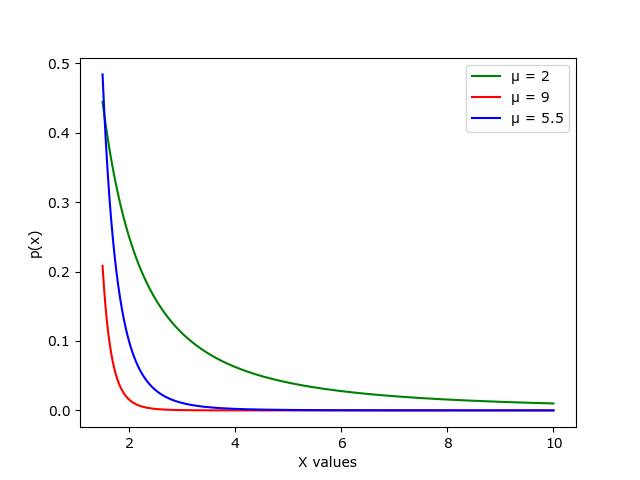
\includegraphics[scale=0.7]{Figure_1}
\end{figure}
\end{document}